%!TEX root=main.tex
\chapter{Work Development} \label{cap:desenvolvimento}

This section presents the work developed thus far, including an overview of the main technologies employed, the implementation of the proposed solution, and its testing and evaluation.

\section{Used Technologies}

The main technologies used in this work are:

\begin{itemize}
    \item \textbf{Programming Language:} To maximize performance while maintaining a reasonable level of abstraction, the implementation was developed in C~\cite{iso_c_2018}, using the intrinsics library to expose vector and cryptographic instructions provided by the ARM architecture~\cite{arm_neon_intrinsics};
    \item \textbf{OpenMP:} Enables the exploitation of thread-level parallelism with minimal modifications to the sequential code, allowing the implementation to take advantage of the multicore capabilities of the ARM Cortex-A55 processor.
\end{itemize}

\section{Project and Implementation}

In this section, we discuss our CKKS implementation, focusing on the operations performed on the client side. First, on the algorithmic level and after on the software implementaton level considering the target architecture characteristics

\subsection{Algorithmic Analysis and Implementation}

First, we describe our implementation of each client-side operations, focusing on the algorithmic level and without discussing operation-level or architectural optimizations.

\subsubsection{Key and Parameter Generation}

From the user point of view the key generation and parameter generation are only one, which must be executed once per scheme instance. Therefore, they will be discussed jointly in this section.

\paragraph{Parameter Generation}

At the beginning of the process, the user provides either the minimum configuration set $(n', \Delta, L, \lfloor \log_2 q_0 \rfloor)$, or the complete configuration set $(n', \Delta, L, n, (q_0, q_1, \ldots, q_L))$.

For the minimum configuration, the client application determines $n$ based on the specified value of $\lfloor \log_2 q_0 \rfloor$, using the lookup table proposed by~\cite{al2022openfhe} to guarantee 128-bit security. Subsequently, the client application generates the modulus chain by starting from $2^{\lfloor \log_2 q_0 \rfloor} + 2^{\lfloor \log_2 q_0 \rfloor-1}$ and testing successive integers of the form $2^{2n}c + 1$ until all required prime moduli are found. Primality is tested using the Miller--Rabin primality test~\cite{Rabin1980}.

For both configuration scenarios, the client computes a $2n$-th primitive root of unity for each modulus $q_i$. Rather than directly searching for an element $\alpha_i$ satisfying $\alpha_i^{2n} \equiv 1 \pmod{q_i}$ and $\alpha_i^n \equiv -1 \pmod{q_i}$, we exploit Fermat's Little Theorem~\cite{HardyWright1979}. For each prime $q_i$ and $0 < \beta < q_i$, Fermat's Little Theorem guarantees that $\beta^{q_i-1} \equiv 1 \pmod{q_i}$. Since $2n \mid (q_i-1)$, if $\beta$ is a $q_i-1$-th primitive root modulo $q_i$, then a $2n$-th primitive root of unity can be obtained as $\alpha \equiv \beta^{(q_i-1)/2n} \mod q_i$. To identify a $q_i-1$-th primitive root $\beta$, it is sufficient to verify that $\beta^{p_j} \not\equiv 1 \mod q_i$ for every distinct prime factor $p_j$ of $q_i-1$. The prime factorization of $q_i-1$ is obtained using the Brent--Pollard Rho factorization algorithm~\cite{Brent1980}. Since both the server and the client must use the same set of roots, we compute all $2n$ powers of $\alpha$ and select the smallest positive value greater than $1$ among them as the canonical representative of $\alpha$. Furthermore, the first $n$ of the $2n$ primitive roots of $\mathbb{C}^{\frac{n}{2}}$are computed as: $w_i = e^{i\pi/2n}$. 

Moreover, we need to construct an XOF to generate the pseudorandom sequences used by our sampling routines. In our implementation, we use AES-128 in counter (CTR) mode as the XOF, as specified in Section~\ref{work:aes}. Specifically, the pseudorandom sequence is generated by encrypting successive values of a counter under AES-128. Consequently, during parameter generation, we also sample a random 128-bit value, which is used as the AES-128 key, and generate the AES round keys. This provides a 128-bit security level, consistent with our security requirement~\cite{stallings2014network}.

\paragraph{Key Generation}

First, we generate the secret key $S$ from a ternary sampling and store it into the original and \textbf{doubleCRT} formats, as both formats are required by subsequent operations.

%. As explained in Section~\ref{ckks:client}, we use an XOF to generate a pseudorandom sequence. We process the sequence in groups of two bits and interpret each group as an integer in $\{0,1,2,3\}$. If the value is smaller than $3$, it is accepted and mapped to an element of $\{-1,0,1\}$; otherwise, it is discarded. The generated secret key $S$ is stored in both original and \textbf{doubleCRT} formats, as both formats are required by subsequent operations.

%Assuming that the output of the XOF is uniformly distributed, each two-bit group is discarded with probability $1/4$. Therefore, to generate $n$ coefficients, we initially request $4\lceil n/3\rceil$ bits from the XOF. If the generated sequence is exhausted before all coefficients have been obtained, additional bits are requested from the XOF and the process continues until the secret key is fully generated.

From $S$, we can derive the public key (RLWE(0)), the conjugation key ($S^{-1}$), the relinearization key ($S^2$), the rotations keys ($S^{5^1}, S^{5^2}, S^{5^4}, \cdots , S^{5^{n/2-1}}$). Except for the public key, all of these keys are stored in gadget decomposition format, as described in Section~\ref{ckks:ops}. For rotations, we store only $\log_2 n - 1$ power-of-two rotation keys. Consequently, an arbitrary rotation may be decomposed into $1$ to $\log_2 n-1$ successive rotations by powers of two, depending on the binary representation. Since each rotation key is relatively large and is stored in gadget decomposition format, this approach introduces a trade-off between memory consumption and performance.

\subsubsection{Encryption}

Following the procedure described in Section~\ref{ckks:encrypt}, given a slot vector $v$, we first encode and expand it to obtain the plaintext $\Delta M$. To encrypt the plaintext, we first generate the error polynomial \(E\) and the uniform polynomial \(A\). %In both cases, we first generate a pseudorandom sequence using the XOF and then transform it into samples from the desired distribution, similarly to the procedure used to generate the secret key \(S\).
%For the error polynomial \(E\), we use the set \(\{-24,\ldots,24\}\), which significantly simplifies the vectorization of this routine, as discussed in Section~\ref{work:arm}. For each output coefficient, we extract two 24-bit values from the pseudorandom sequence, compute the Hamming weight of each value, and subtract the two resulting values. Consequently, the XOF only needs to generate \(48n\) bits of data, since no rejection is performed.
Then, \(E\) is added to \(\Delta M\), and the resulting polynomial is converted to the \textbf{doubleCRT} representation.

%For the uniform polynomial \(A\) over \(\{0,1,\ldots,p-1\}\), where \(p\) is prime, we perform the sampling directly in the NTT domain, eliminating the need for an additional NTT conversion. Since the polynomial and the NTT domain are homomorphic, this simplification is valid. Similar to the generation of the secret key \(S\), we extract a fixed number of bits from the pseudorandom sequence and accept or reject the resulting value according to a predefined threshold. Because the moduli chain may vary between CKKS instances, tailoring the implementation to a specific modulus is undesirable. Instead, for each coefficient, we sample a 64-bit value and accept it if $p\lfloor(2^{64}-1)/p\rfloor$. The accepted value is then reduced to the range \(\{0,1,\ldots,p-1\}\) using the Barrett reduction method described in Algorithm~\ref{background::math::barret}.

\subsubsection{Decryption}

The decryption procedure follows directly from the method described in Section~\ref{ckks:decrypt}. In our implementation, only the component corresponding to the remaining modulus \(q_0\) of the received ciphertext \(c\) is decrypted and decoded to recover the slot vector \(v\).

\subsection{ARMv8 Implementation}
\label{work:arm}

In this section, we will describe how the main primitives of our client-side CKKS operations are implemented considering the characteristics of the ARM Cortex-A55.

\subsubsection{AES-CTR}
\label{work:aes}

Since our security requirements specify a computational security level of 128 bits, we restrict our AES-CTR implementation to AES-128. The implementation is divided into two main components: pseudorandom data generation and round-key generation.

\paragraph{Pseudorandom data generation}

The pseudorandom data generation exploits the vector AES instructions available on the target core. To perform an AES encryption round, the \texttt{vaese} and \texttt{vaesmc} instructions are combined to apply the \textbf{AddRoundKey}, \textbf{SubBytes}, \textbf{ShiftRows}, and \textbf{MixColumns} transformations to a vector register representing the AES state. Specifically, \texttt{vaese} performs the \textbf{AddRoundKey}, \textbf{SubBytes}, and \textbf{ShiftRows} transformations, while \texttt{vaesmc} performs \textbf{MixColumns}. By combining these instructions, the AES round transformations can be efficiently implemented using dedicated hardware support.

To exploit data-level parallelism and reduce control overhead, the implementation processes eight AES states concurrently, without causing vector register spilling. This parallelization is possible because each output block is generated independently by encrypting a distinct counter value under the same key. Consequently, the eight counter blocks can be processed simultaneously. %, allowing the implementation to better utilize the available vector execution resources while improving throughput.

\paragraph{Round-key generation}

This stage is considerably more complex than pseudorandom data generation because there is no direct correspondence between the processor instructions and the operations defined by the AES key expansion algorithm. The vectorization strategy adopted in this work is illustrated in Figure~\ref{fig::aes_round}. As in the AES specification, the matrix elements in the figure are arranged in column-major order.

To compute the word \(w' = \operatorname{SubWord}(\operatorname{RotWord}(w_{i-1})) \oplus \operatorname{Rcon}[i/N_k]\), we first apply the \texttt{vaese} instruction to the state matrix \(a\), which contains the previous round key, using an auxiliary zero vector as the round key. This operation applies the \textbf{SubBytes} and \textbf{ShiftRows} transformations while effectively neutralizing \textbf{AddRoundKey}. Since \textbf{ShiftRows} is not required for the key expansion, its effect is subsequently reversed using the \texttt{vqtbl1} instruction, which also implements the required byte permutation. This approach allows us to reuse the hardware-accelerated AES instructions to perform the SubWord transformation.

Next, we use the \texttt{vset\_lane} instruction to insert the appropriate round-constant byte into a zero vector, placing it at the position corresponding to the required \(\operatorname{Rcon}\) value. We then apply the \texttt{veor} instruction to XOR this vector with the intermediate result, introducing the round constant only at the desired position. Finally, the \texttt{vqtbl1} instruction applies the required byte permutation, reverses the \textbf{ShiftRows} rearrangement, and replicates the resulting word across the four columns of the vector register, completing the computation of \(w'\).

The remaining key expansion operations require XORing each column of \(a\) with its preceding columns. We implement this process in two stages using the \texttt{vext} and \texttt{veor} instructions. In the first stage, \texttt{vext} rearranges the vector elements to align each column with its predecessor, and \texttt{veor} computes their pairwise XOR. In the second stage, the same approach is applied to combine each column with the corresponding intermediate result from two columns earlier. This two-stage process efficiently computes the cumulative XOR operations required by the AES key expansion algorithm. Finally, we XOR the resulting vector with \(w'\), replicated across all four columns, to generate the new round key \(f\).

\begin{figure}
    \centering
    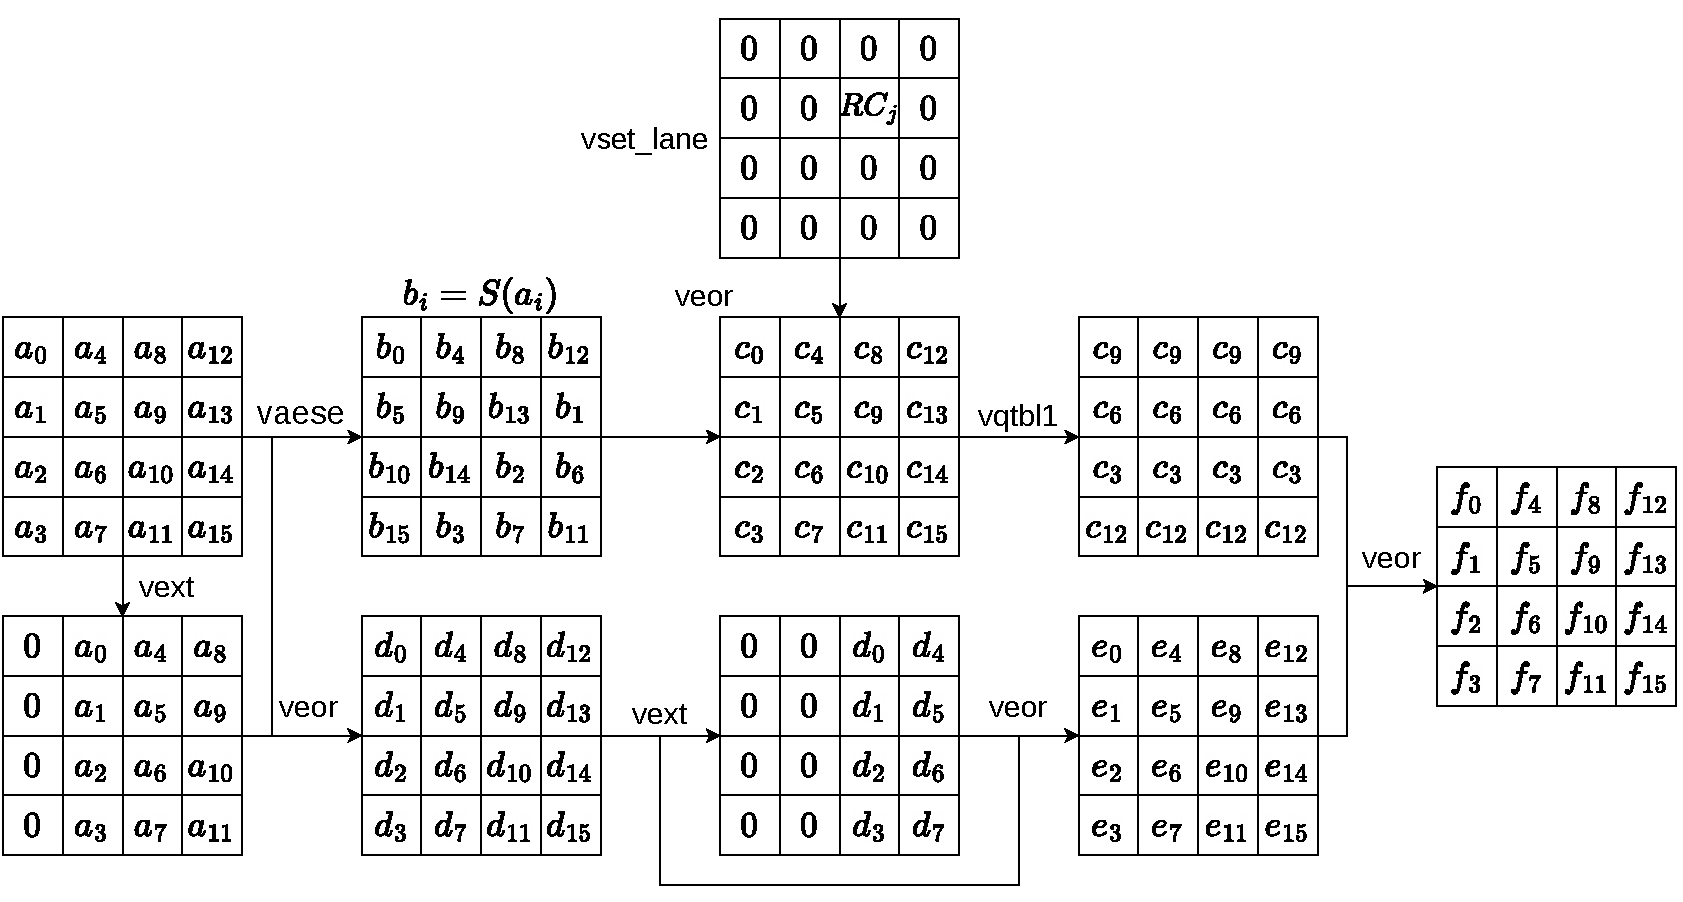
\includegraphics[width=1\linewidth]{Images/AES-Round-Key.pdf}
    \caption{AES Round-Key Generation $f$ from the previous round-key $a$ using ARM NEON instructions. $RC_j = \text{RCon}[i/N_k]$. $S$: Application of \textbf{SubBytes}.}
    \label{fig::aes_round}
\end{figure}


\subsubsection{Sampling Procedures}

Our CKKS implementation includes three main sampling routines: ternary sampling, binomial sampling, and uniform sampling. All three routines first generate a sequence of pseudorandom bytes using AES-CTR and then derive samples from the desired probability distribution using this sequence.

\paragraph{Ternary and Uniform Sampling}

For ternary and uniform sampling, we use rejection sampling: candidate values outside a specified range are discarded, while those within the range are accepted. If the initial byte sequence does not yield enough samples, additional pseudorandom bytes are generated. To minimize calls to the AES-CTR routine, we initially generate enough bytes to produce the required number of samples in expectation, accounting for the rejection probability under the assumption that the pseudorandom bytes are uniformly distributed.

For ternary sampling, we partition the byte sequence into 2-bit values. Values equal to three are rejected, while the remaining values are converted in constant time to the 64-bit integers $-1$, $0$, and $1$. For uniform sampling, the modulus $q$ is known only at runtime. We therefore partition the byte sequence into 64-bit candidates and accept a candidate if it is smaller than the rejection threshold ($2^{64}-1-((2^{64}-1) \bmod q)$). The accepted candidate is then reduced modulo $q$, using the Barrett reduction method, to obtain a uniformly distributed sample.

Since ARM NEON does not directly support predicated vector operations for this rejection process, the conditional acceptance and rejection of individual candidates cannot be efficiently implemented using vector instructions. Consequently, we do not vectorize either of these sampling routines.

\paragraph{Binomial Sampling}

For binomial sampling, we generate values from the set $\{-24, \ldots, 24\}$ according to the desired binomial distribution. Given two 24-bit values, $a$ and $b$, a sample can be computed by subtracting their population counts $x = \operatorname{popcount}(a) - \operatorname{popcount}(b)$. Thus, for a polynomial of $n$ coefficients, we can generate the required pseudorandom input using $6n$ bytes and derive all samples directly, without requiring additional random values.

Our target architecture provides a dedicated instruction, \texttt{vcnt}, to compute the population count of 8-bit elements in vector registers, enabling us to vectorize this routine. However, the kernel involves mixed-width arithmetic: population counts are computed on 8-bit elements, whereas the final results are 64-bit integers obtained by subtracting the population counts of two groups of three bytes.

To minimize the number of conversion and permutation instructions required to handle this mixed-width arithmetic, we divide the $6n$-byte sequence into six consecutive segments, each containing $n$ bytes. The $i$-th sample is computed from the $i$-th byte of each segment, with the first three bytes contributing to one population count and the remaining three to the other. This arrangement allows us to perform memory accesses and intermediate arithmetic using element-wise operations, removing data rearrangement overhead and making more effective use of the vector execution pipeline.

\subsubsection{Modular Arithmetic}

Modular arithmetic involves two fundamental operations: addition and multiplication. Both require modular reduction to ensure that the results remain within the desired range. As discussed in Section~\ref{ckks:cte_red}, these reductions must be implemented in constant time to prevent timing side-channel attacks.

For modular addition, we employ Barrett reduction. To reduce the frequency of modular reductions, we restrict the moduli to 63 bits, which is less restrictive than the 62-bit limit adopted by Intel HEXL, a high-performance library for homomorphic encryption arithmetic~\cite{boemer2021intel}. This restriction allows us to perform two consecutive modular additions before applying a reduction, as the intermediate results remain within the representable range of the integer data type. Consequently, we reduce the number of modular reduction operations without risking integer overflow.

For modular multiplication, we employ Montgomery multiplication. However, this approach introduces an additional consideration: managing the factor \(R\) inherent to Montgomery arithmetic. On the client side, modular multiplications occur primarily during the NTT and when multiplying the secret key \(S\) by the uniformly sampled polynomial \(A\) during encryption and decryption. We exploit the structure of these operations to eliminate the overhead associated with explicitly handling the Montgomery factor.

During the NTT, polynomial elements are repeatedly multiplied by primitive roots of unity. Since these roots are computed during parameter generation, we precompute and store them in Montgomery representation, effectively incorporating the factor \(R\) into each root. This allows the \(R^{-1}\) factor introduced by Montgomery multiplication to be canceled, avoiding the need for additional conversions during the transform. For polynomial multiplication involving \(A\), we exploit the fact that its coefficients are sampled uniformly. Multiplication by \(R\) modulo \(q\), provided that \(R\) is invertible modulo \(q\), preserves the uniform distribution. Therefore, we can equivalently represent the coefficients of \(A\) in Montgomery form without compromising their uniformity or introducing additional security concerns. This approach eliminates the need for explicit conversions when multiplying \(A\) by the secret key.

Furthermore, Montgomery multiplication allows us to combine a multiplication with a preceding addition, postponing modular reduction and avoiding the need to reduce the intermediate sum separately, provided that the intermediate values remain within the supported arithmetic range.

Alternative modular multiplication algorithms, such as Plantard multiplication~\cite{plantard2021efficient}, can reduce the number of arithmetic instructions required compared with Montgomery multiplication. However, CKKS implementations are often memory-bound~\cite{kim2022ark}, making memory traffic a critical performance consideration. Some alternative methods require additional precomputed constants depending on the operands value, increasing memory-access requirements. We therefore favor Montgomery multiplication, as it offers a suitable balance between computational efficiency and memory usage for our target architecture.

\subsubsection{NTT and INTT}
\label{work::arm::ntt}

Since ARMv8 does not provide vector instructions for 64-bit integer arithmetic on the target architecture, we chose not to vectorize this operation. Simulating 64-bit multiplication using 32-bit instructions requires at least seven arithmetic instructions per operation: four multiplications and three additions. Given that each vector register can accommodate four 32-bit elements, the maximum theoretical performance gain from vectorization is \(4\times\). Consequently, the overhead of emulating 64-bit arithmetic would likely outweigh the benefits of vectorization, leading us to focus on optimizing the scalar implementation instead.

A well-known technique for accelerating the Cooley–Tukey (CT) and Gentleman–Sande (GS) algorithms is to exploit their in-place computation to merge multiple stages into a single processing block. Instead of loading and storing the polynomial elements at every stage, this approach loads the required elements into registers, performs several consecutive stages, and stores the results only after all merged stages have been completed. This technique, commonly referred to as stage merging, reduces memory accesses and loop-control overhead, thereby improving performance.

However, the polynomial degree \(n\) is known only at runtime. To avoid code-size growth and maintenance problems, we do not want to generate a separate implementation for every valid value of \(n\). Instead, we aim to develop a single implementation that efficiently exploits stage merging while accommodating the stage-dependent permutation patterns and the runtime variability of \(n\).

Another critical aspect of stage merging is determining the optimal number of stages to combine. Merging \(\ell\) consecutive stages requires simultaneously storing \(2^\ell\) polynomial elements in registers. Since the target architecture provides only 32 general-purpose registers, which must also accommodate primitive roots, pointers, and other values required for program execution, the number of merged stages must be carefully selected to avoid register spilling. Spilling registers to memory can significantly increase memory traffic and negate the performance benefits of stage merging.

For CT-NTT, GS-INTT follows an analogous approach, we begin by merging the final four stages, which requires 16 registers to hold the polynomial elements. Merging five stages would require 32 registers for these elements alone, leaving no registers available for other purposes and inevitably causing register spilling. In this final four-stage group, the permutation size ranges from 1 to 8 elements. Consequently, the 16 elements required by each block occupy consecutive positions in the polynomial, allowing them to be loaded into registers using a blocked access pattern.

For the remaining stages, we merge three consecutive stages at a time. Each such group requires eight registers for the polynomial elements and seven registers for the corresponding primitive roots. This arrangement allows the primitive roots to be loaded outside the innermost loop, eliminating their repeated acquisition during the processing of individual elements. Merging additional stages would increase register pressure to 31 registers for the polynomial elements and primitive roots alone, leaving insufficient capacity for the remaining variables and causing register spilling. In these groups, the permutation size ranges from \(2^\ell\) to \(2^{\ell-2}\), where \(\ell>5\). Since the permutation size exceeds the eight elements processed simultaneously, the elements belonging to a given block are distributed across the polynomial according to an interleaved pattern rather than occupying consecutive positions.

However, because \(n\) is known only at runtime, the number of stages preceding the final four may not be divisible by three. Therefore, merging groups of three stages alone cannot handle every valid value of \(n\). To address this issue, we adapt the initial stages according to the remainder of \(\log_2 n-4\) modulo three. Specifically, when \(log_2 n-4 \equiv 0 \pmod 3\), all preceding stages can be merged in groups of three. When \(log_2 n-4 \equiv 1 \pmod 3\), the first stage is executed separately before merging the remaining stages in groups of three. Finally, when \(log_2 n-4 \equiv 2 \pmod 3\), the first two stages are merged together, followed by groups of three stages. This strategy accommodates the runtime-dependent number of stages while preserving the benefits of stage merging.

Figure~\ref{fig::ct_scalar} illustrates the proposed stage-merging strategy for the CT-NTT with \(n=256\). Elements belonging to the same block are loaded into registers and processed within the same inner-loop iteration. Since \((\log_2 256-4)\bmod 3=1\), the first stage is executed separately. Stages 2, 3, and 4 are then merged and processed in \(256/8=32\) blocks. For each block, the corresponding elements follow an interleaved pattern, with indices determined by the permutation pattern of the merged stages. Finally, stages 5 through 8 are merged and processed in \(256/16=16\) blocks, each containing 16 consecutive polynomial elements. This final group uses a blocked access pattern because the elements required by the merged stages occupy contiguous positions in the polynomial.

\begin{figure}
    \centering
    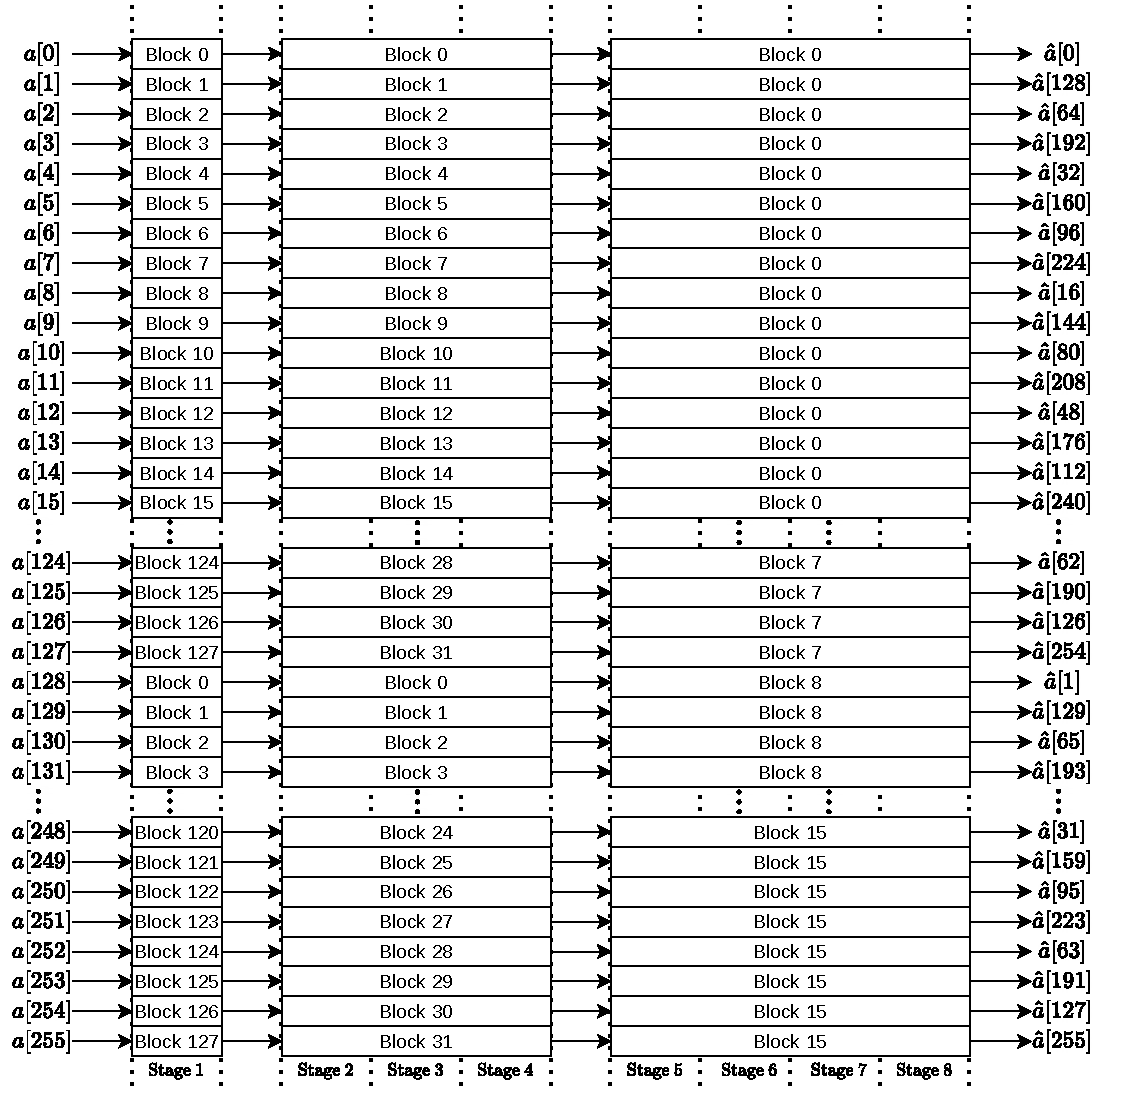
\includegraphics[width=1\linewidth]{Images/Merge-CT-Scalar.pdf}
    \caption{Stage-merging strategy for the scalar CT-NTT with $n=256$.
    Elements belonging to the same block are loaded into registers and
    processed within the same inner-loop iteration. Stages 2--4 are merged
    using an interleaved access pattern, whereas stages 5--8 are merged
    using a blocked access pattern.}
    \label{fig::ct_scalar}
\end{figure}

\subsubsection{DFT and IDFT}

Unlike the NTT and INTT implementations discussed in Section~\ref{work::arm::ntt}, which are constrained by the lack of vector instructions for 64-bit integer arithmetic, the DFT and IDFT routines can exploit the hardware support for double-precision floating-point operations provided by the target architecture. Since each ARM NEON vector register is 128 bits wide, it can accommodate two double-precision floating-point values, allowing two vector elements to be processed simultaneously.

Another advantage of ARM NEON is its support for vector-scalar arithmetic, which enables operations between a vector register and a scalar value held in a general-purpose register or transferred from a scalar register file, depending on the instruction. This capability provides additional flexibility when implementing our stage-merging strategy. In particular, primitive roots can be maintained in scalar registers and multiplied by multiple vector elements that share the same root at a given stage, reducing redundant loads and improving register utilization.

A key difference between the NTT and DFT implementations lies in the arrangement of the primitive roots. To support slot rotations in the polynomial domain, the roots are rearranged so that, within a given stage, they follow an interleaved access pattern rather than the blocked pattern used by the NTT. Consequently, root selection becomes dependent on the current element, requiring root accesses in the innermost loop. Although this arrangement can increase memory-access overhead, it also reduces register pressure because primitive roots do not need to remain in registers across multiple loop iterations.

For the GS-IDFT, it follows an analogous strategy because it shares the same permutation pattern as the CT-NTT, as explained in Section~\ref{ckks::convert}. We begin by merging the final four stages, which requires 16 vector registers to hold the vector elements. Merging five stages would require 32 registers for the vector elements alone, leaving no registers available for intermediate values and inevitably causing register spilling. Within this four-stage group, the permutation size ranges from 1 to 8 elements. Therefore, the 16 elements processed by each block occupy consecutive positions in the vector and can be loaded using a blocked access pattern. However, when the permutation size is one, the required permutation involves exchanging elements within and across vector registers. We implement this rearrangement using a combination of the \texttt{vzip1} and \texttt{vzip2} instructions.

For the preceding stages, we merge three consecutive stages at a time. Rather than distributing the vector elements using a fully interleaved pattern, we adopt a mixed interleaved-blocked layout, in which interleaving occurs between pairs of consecutive elements. This arrangement allows consecutive elements to be loaded together into vector registers, improving load-store unit utilization while avoiding additional permutation instructions. However, this strategy already requires 16 vector registers to hold the vector elements, leaving insufficient register capacity to merge another stage without register spilling.

Primitive roots are handled separately from the vector elements. Depending on the stage and the available register capacity, they are either maintained in scalar registers and used directly by vector-scalar arithmetic instructions or loaded into a limited number of vector registers. This approach allows the implementation to exploit the available scalar and vector resources while avoiding register spilling.

As in the NTT and INTT implementations, the slot-vector size is known only at runtime, requiring the initial stages to be handled according to the number of stages that can be merged. We use the same general strategy described in Section~\ref{work::arm::ntt}, adapting the initial stages to accommodate the runtime-dependent size. However, we retain the mixed interleaved-blocked layout for these stages, using 16 vector registers to hold the vector elements. Consequently, merging a single stage implies loading eight consecutive elements, whereas merging two stages lead to load four consecutive elements. This approach maintains a consistent memory-access pattern while accommodating different slot-vector sizes.

Figure~\ref{fig::gs_vector} illustrates the proposed stage-merging strategy for the GS-IDFT with \(n=256\). Elements belonging to the same block are loaded into registers and processed within the same inner-loop iteration. The implementation processes 32 blocks, each containing eight vector registers, corresponding to 16 double-precision elements. In Stage 1, the elements are distributed using an interleaved pattern across groups of eight consecutive elements. For Stages 2–4, the mixed interleaved-blocked layout is applied between pairs of consecutive elements. Finally, Stages 5–8 use a blocked layout, in which each block contains 16 consecutive polynomial elements.

%Since \((\log_2 256-4)\bmod 3=1\), the first stage is executed separately. Stages 2, 3, and 4 are then merged and processed in \(256/16=16\) blocks. For each block, the corresponding elements follow an interleaved pattern, with indices determined by the permutation pattern of the merged stages. Finally, stages 5 through 8 are merged and processed in \(256/16=16\) blocks, each containing 16 consecutive polynomial elements. This final group uses a blocked access pattern because the elements required by the merged stages occupy contiguous positions in the polynomial.

\begin{figure}
    \centering
    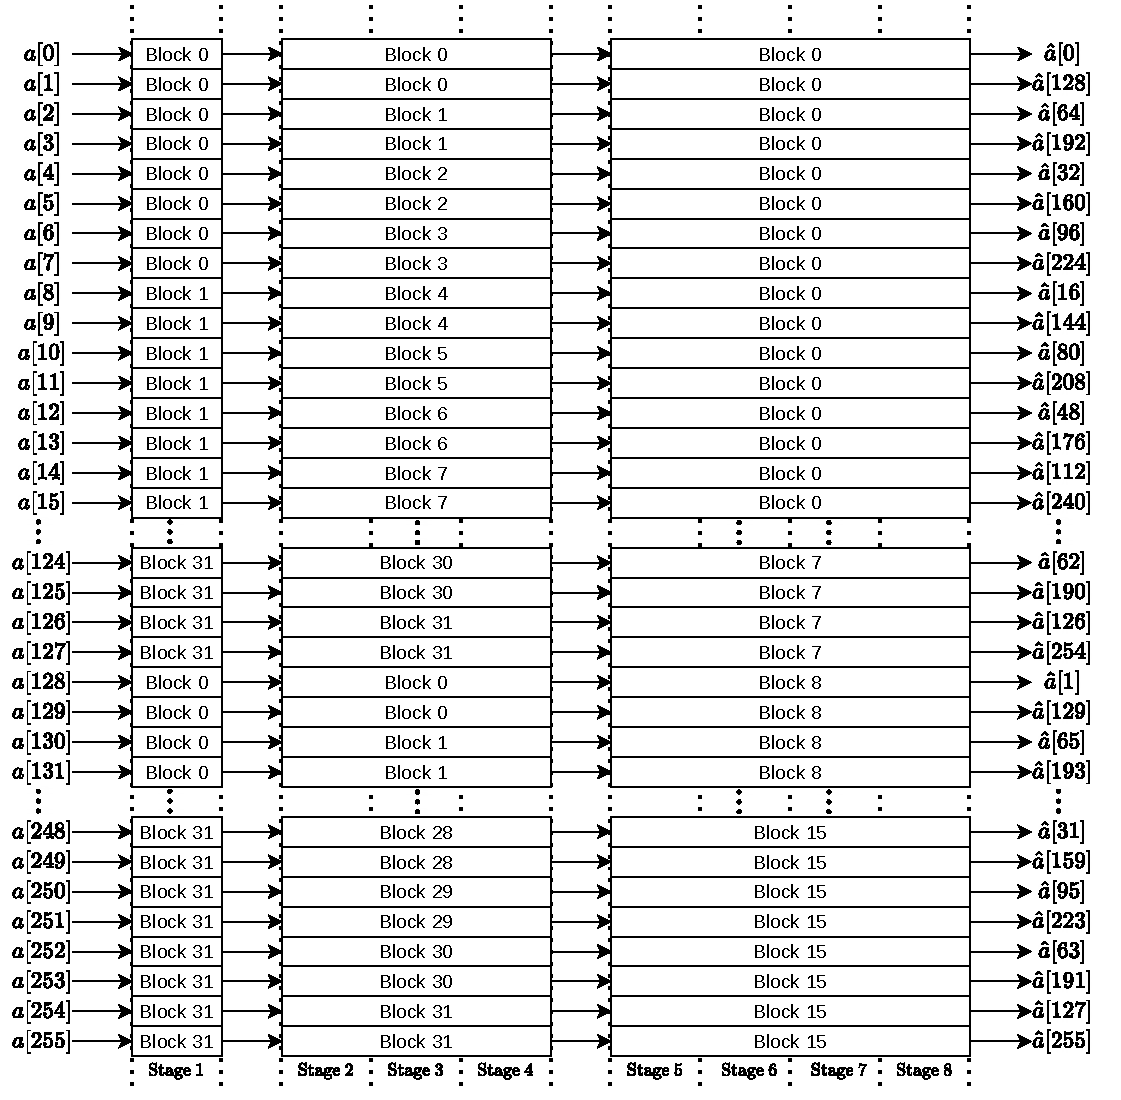
\includegraphics[width=1\linewidth]{Images/Merge-GS-Vector.pdf}
    \caption{Stage-merging strategy for the scalar GS-IDFT with $n=256$.
    Elements belonging to the same block are loaded into registers and
    processed within the same inner-loop iteration. Stage 1 and Stages 2--4 are merged
    using a mixed interleaved-blocked access pattern, whereas stages 5--8 are merged
    using a blocked access pattern.}
    \label{fig::gs_vector}
\end{figure}

\section{Testes e Avaliação}
Descrever o procedimento da avaliação do trabalho (teste de hardware, teste de software, teste de módulo, teste de integração, teste de validação), de acordo com o tipo do sistema, com o apoio do orientador, se necessário.